%\VignetteIndexEntry{Getting started with the package}
%\VignetteKeywords{getting started}
%\VignettePackage{surveillance}

\documentclass[a4paper,11pt]{article}
\usepackage{natbib}
\bibliographystyle{apalike}

% Preabmle parts
\usepackage[T1]{fontenc}        % Make it possible to use danish characters !!
\usepackage{url}
\usepackage{hyperref}
\usepackage{times}  
\renewcommand{\sfdefault}{ptm} % Brug times som font - vigtigt i
                               % pdflatex?

%PSTricks
\usepackage{pdftricks}
\begin{psinputs}
  \usepackage{pst-all}
\end{psinputs}

\usepackage{bm}
\usepackage{amsmath}
\usepackage{amssymb}
\usepackage{latexsym}
\usepackage{verbatim}
\usepackage{relsize}
\usepackage{epsfig}
\usepackage{comment}
\newcommand{\surveillance}{\texttt{surveillance}}
\usepackage{pdfpages}
\setlength{\parindent}{0pt} 



\title{The function 'algo.glrnb' in the R-Package 'surveillance'}
\author{
Valentin Wimmer$^{(1,2)}$\thanks{Author of correspondence: Email: \texttt{Valentin.Wimmer@gmx.de}}$\>\>$ and Michael H�hle$^{(1,2)}$ \\
(1) Department of Statistics\\
University of Munich, Germany\\
(2) MC-Health - Munich Center of Health Sciences
} \date{\today}

\usepackage{Sweave}
\begin{document}
%%%%%%%%%%%%%%%%%%%%%%%%%%%%%%%%%%%%%%%%%%%%%%%%%%%%%%%%%%%%%%%%%%%%%%
% Sweave 
%%%%%%%%%%%%%%%%%%%%%%%%%%%%%%%%%%%%%%%%%%%%%%%%%%%%%%%%%%%%%%%%%%%%%%
%Put all in another directory

 \setkeys{Gin}{width=1\textwidth} 

\DefineVerbatimEnvironment{Sinput}{Verbatim}{fontshape=sl,fontsize=\relsize{-1}}
\DefineVerbatimEnvironment{Soutput}{Verbatim}{fontshape=s1,fontsize=\relsize{-1}}
\DefineVerbatimEnvironment{Scode}{Verbatim}{fontshape=sl,fontsize=\relsize{-1}}


%%%%%%%%%%%%%%%%%%%%%%%%%%%%%%%%%%%%%%%%%%%%%%%%%%%%%%%%%%%%%%%%%%%%%%
% Initial R code
%%%%%%%%%%%%%%%%%%%%%%%%%%%%%%%%%%%%%%%%%%%%%%%%%%%%%%%%%%%%%%%%%%%%%%




\maketitle  
%\mbox{}\hrulefill\\

\begin{abstract}
  \noindent The aim of this document is to show the use of the function \verb+algo.glrnb+ for a type of count data regression chart, the generalized likelihood ratio (GLR) statistic. The function is part of the R-Package '\texttt{surveillance}' \citep{hoehle2007R}, which provides outbreak detection algorithms for surveillance data. For an introduction to this package, the vignette for the package can be used \citep{vignette}. There one can find information about the data structure of the \verb+disProg+ and \verb+SurvRes+ objects. Furthermore tools for outbreak detection, such as a Bayesian approach, procedures described by \citet{stroup89},
  \citet{farrington96} and the methods used at the Robert Koch Institut, Germany, are explained. 
  
  The function \verb+algo.glrnb+ is the implementation of the control charts for poisson and negative binomial distributions for monitoring time series of counts described in \citet{hoehle2008}. This document gives an overview of the different features of the function and illustrations of its use are given for simulated and real surveillance data. \\
  
    \noindent{\bf Keywords:} change-point detection, generalized regression charts, poisson and negative binomial distribution, increase and decrease
\end{abstract}


\section{Introduction}\label{sec:intro}

For the monitoring of infectious diseases it is necessary to monitor time series of routinely collected surveillance data. Methods of the statistic process control (SPC) can be used for this purpose. Here it is important, that the methods can handle the special features of surveillance data, e.g.\ seasonality of the disease or the count data nature of the collected data. It is also important, that not only the number of counts of one time point (week, month) are regarded but instead the cases of previous time points are considered, because beside abrupt changes also small constant changes should be detected. CUSUM-methods (function \verb+algo.cusum+), LR-charts or GLR-methods as described by \citet{lai95} and \citet{hoehle2008} can afford this. With the function \verb+algo.glrnb+ these methods can easily applied to surveillance data.

A typical assumption for time series of counts is, that the observed counts at each time point follow a Poisson distribution. If overdispersion is likely, the negative binomial distribution provides a better alternative. Both distributions are provided by \verb+algo.glrnb+.

In the GLR-scheme, an outbreak can be defined as a change in the intercept. The function \verb+algo.glrnb+ allows the user to specify whether increases or decreases in mean should be regarded. For each time point a GLR-statistic is computed, if this statistic exceeds a threshold value, an alarm is given. The function also provides the possibility to return the number of cases that would have been necessary to produce an alarm.

This vignette is organized as follows: First, in Section \ref{sec:prel} the data structure is explained, in Section \ref{sec:glr} a short introduction in the theory of the GLR-charts is given and Section \ref{sec:control} shows the different \verb+control+-settings. % In Section \ref{sec:extensions} some possible extensions are presented.      


\section{Preliminaries}\label{sec:prel}


Consider the situation, where a time series of counts is collected for surveillance purpose. In each interval, usually one week, the number of cases of the interesting disease in an area (country, district) is counted. The resulting time series is denoted by $\{y_t\>;t=1,\ldots,n\}$. Usually the data are collected on line, so that the time point $n$ is the actual time point. Our aim is to decide with the aid of a statistic for each time point $n$ if there is an outbreak at this or any former time point. If an outbreak is detected, the algorithm gives an alarm. Observed time series of counts are saved in a \verb+disProg+ object, a list containing the time series of counts, the number of weeks and a state chain.  
The state is 1, if e.g. the Robert Koch Institut declares the week to be part of an outbreak and 0 otherwise ~\citep{survstat}. By using the state chain the quality of the surveillance algorithm can be tested.
%The 'surveillance'-package provides standard plot routines for the surveillance objects.
As an first example the number of cases of salmonella hadar in the years 2001-2006 is examined.  \\

\textit{Example 1:}
\begin{Schunk}
\begin{Sinput}
> data(shadar)
> plot(shadar, main = "Number of salmonella hadar cases in Germany 2001-2006")
\end{Sinput}
\end{Schunk}
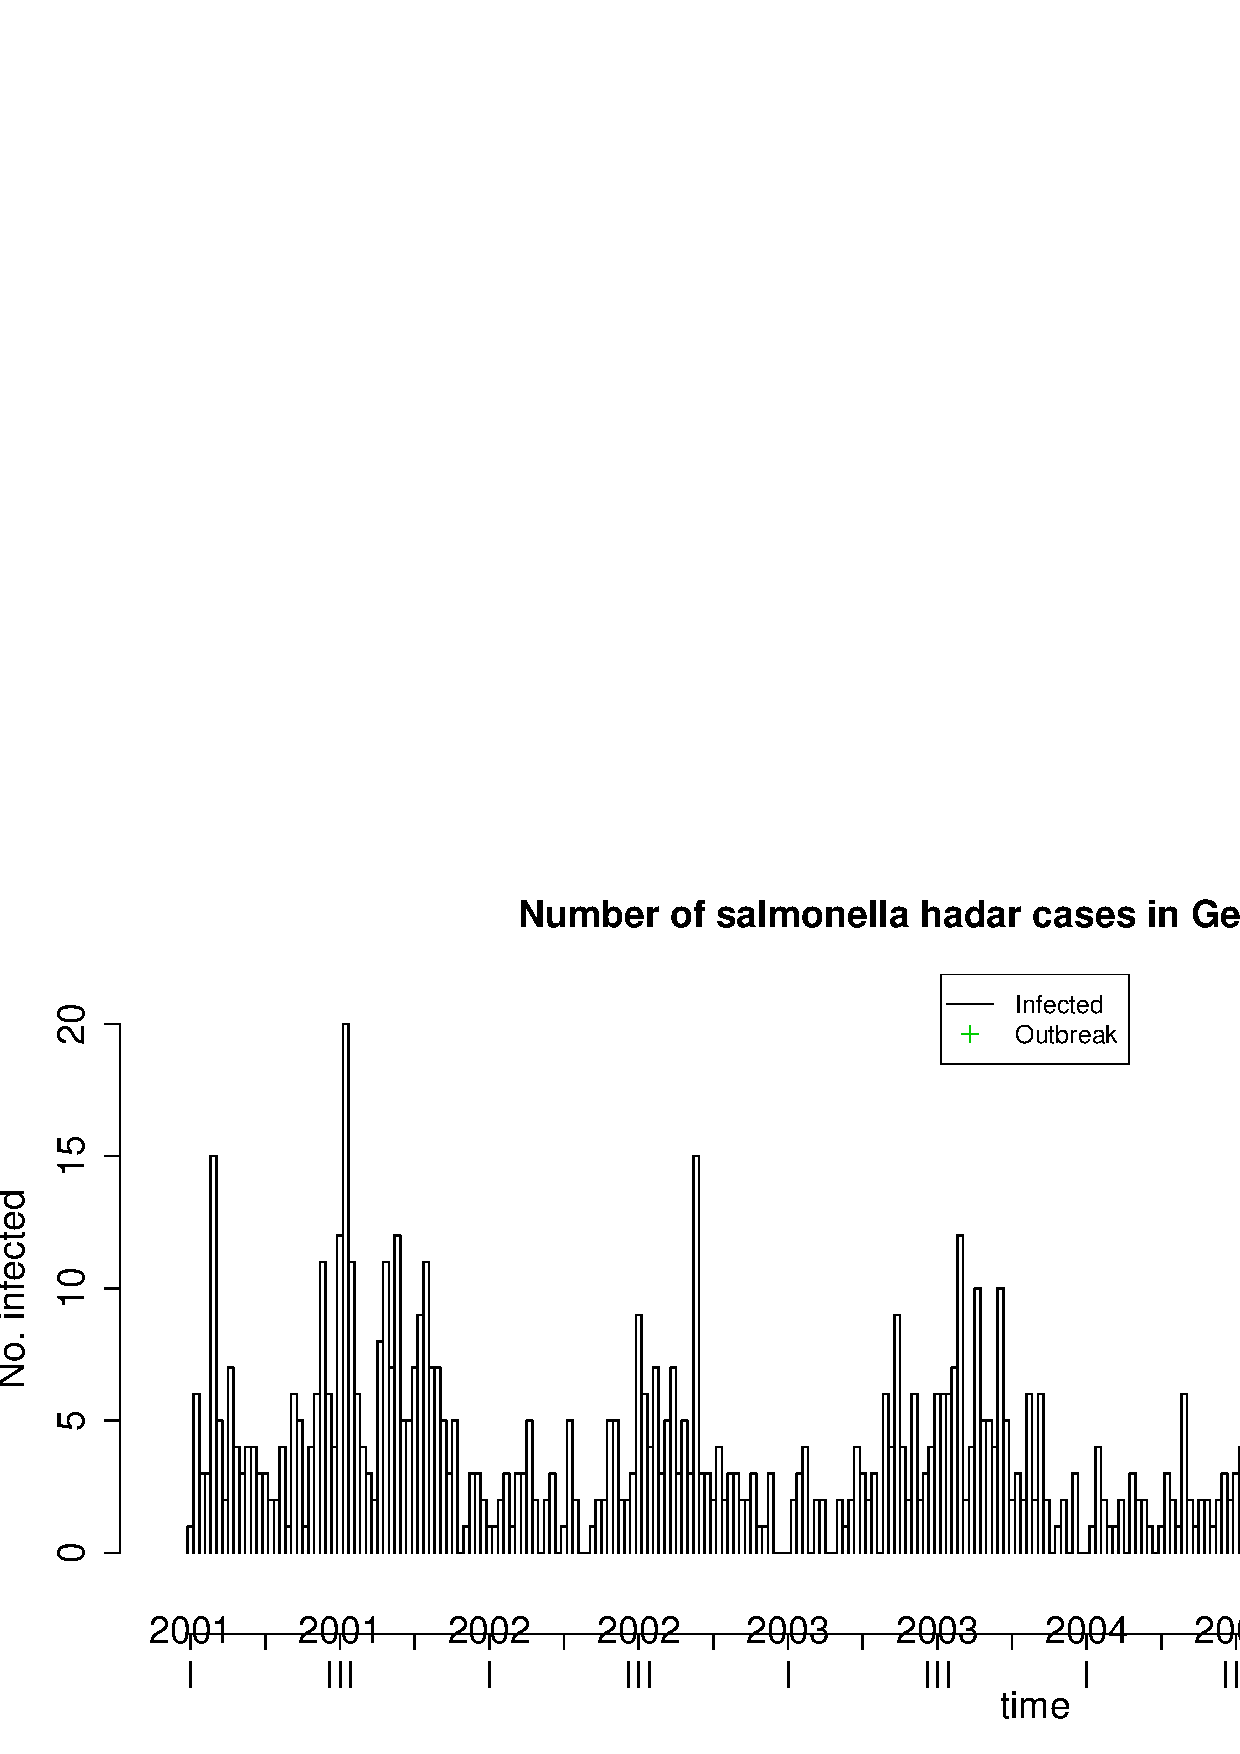
\includegraphics{figs/vignette_glrnb-002}

The package provides the possibility to simulate surveillance data with the functions \verb+sim.pointSource+, \verb+sim.seasonalNoise+ and \verb+sim.HHH+. See \citep{hoehle2007R} and the vignette for further information. \\

\textit{Example 2:}

\begin{Schunk}
\begin{Sinput}
> simData <- sim.pointSource(length = 300, K = 0.5, r = 0.6, 
+     p = 0.95)
\end{Sinput}
\end{Schunk}

\begin{Schunk}
\begin{Sinput}
> plot(simData)
\end{Sinput}
\end{Schunk}
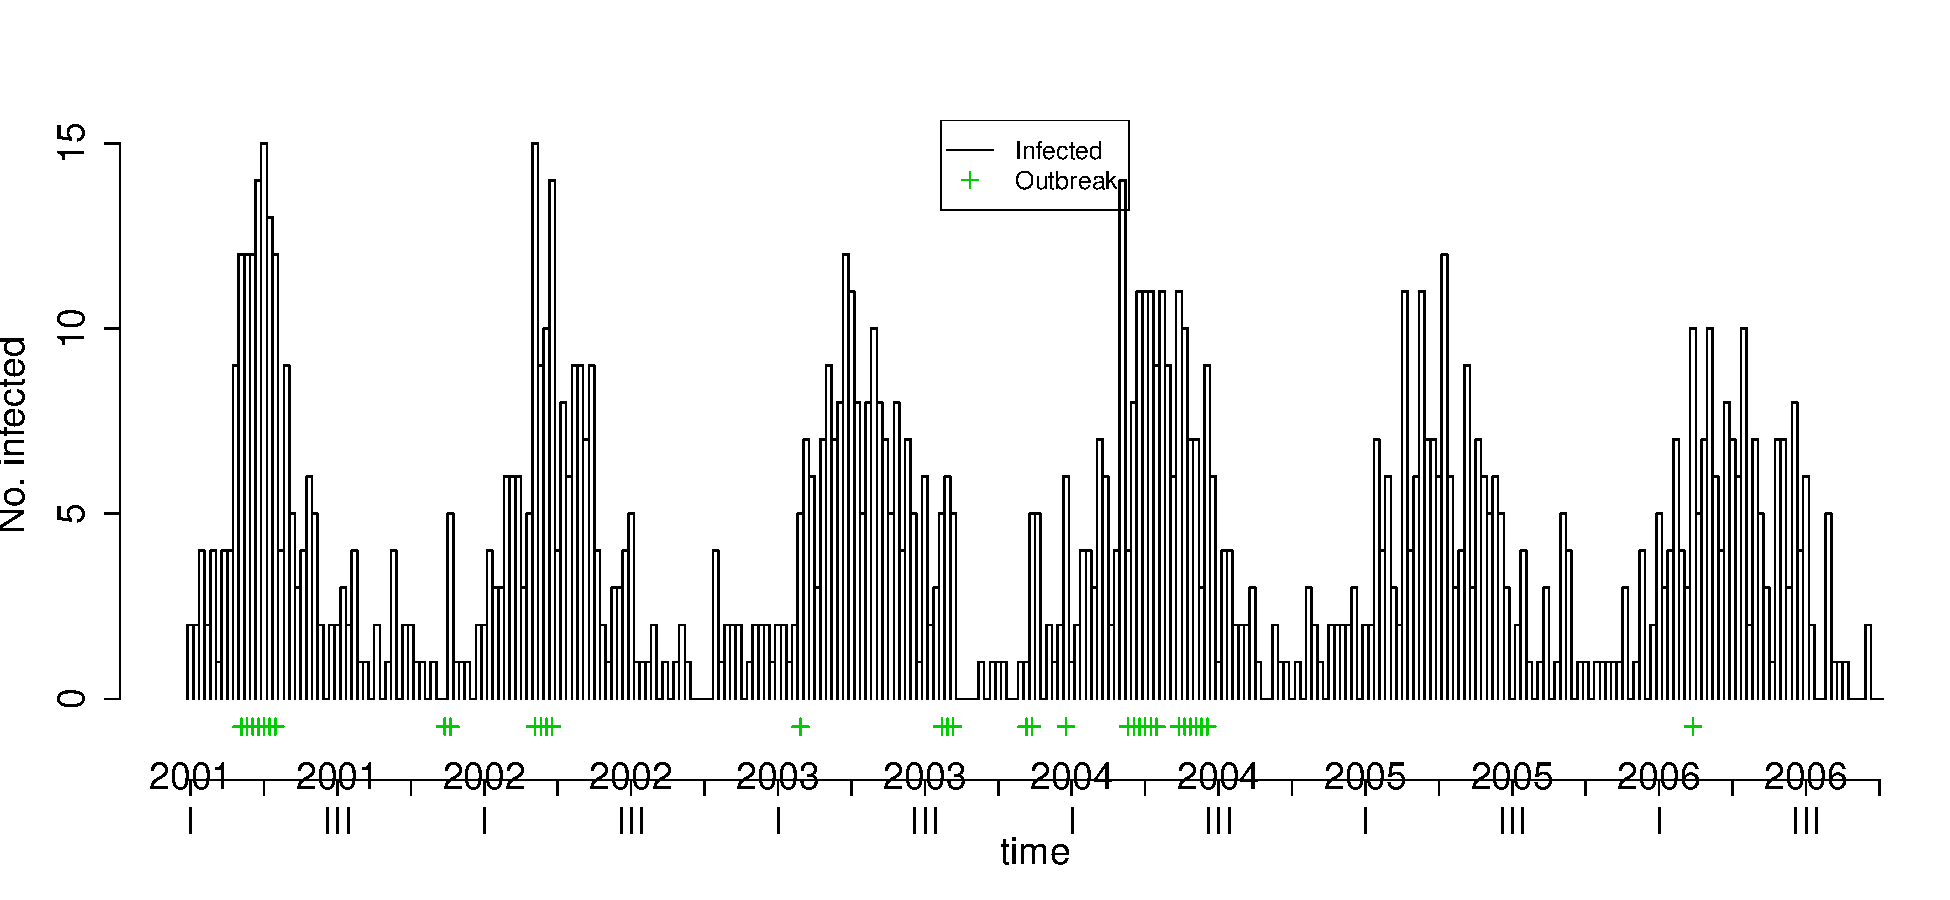
\includegraphics{figs/vignette_glrnb-004}

\section{LR and GLR-charts}\label{sec:glr}


Our aim is to detect a significant change in the number of cases. This is done as follows. One assumes, that there is a number of cases that is usual, the in control mean $\mu_0$. The in-control mean is defined in \citet{hoehle2008} to be
\begin{equation} \label{mu0}
\operatorname{log}(\mu_{0,t})=\beta_0 + \beta_1t + \sum_{s=1}^S(\beta_{2s} \cos(\omega s t) + \beta_{2s+1}\sin(\omega s t)).
\end{equation}

If an outbreak occurs, the number of cases increases and the situation is out-of control and the algorithm should produce an alarm. The change is assumed to be an additive increase on log scale,

\begin{equation} \label{interceptchange}
\operatorname{log}(\mu_1)= \operatorname{log}(\mu_0) + \kappa .
\end{equation}

If $\mu_0$ is unknown one could use a part of the data to estimate it with a generalized linear model (GLM). If $\kappa$ is known, LR-charts can be used, if not, $\kappa$ has to be estimated, which is the GLR-scheme setting. For each time point, the likelihood ratio statistic is computed as follows
\begin{equation}
\label{cusum}
GLR(n)=\max_{1 \leq k \leq n} \sup_{\theta \in \Theta} \left[ \sum_{t=k}^n \log
\left\{ \frac{f_{\theta}(y_t)}{f_{\theta_0}(y_t)}
\right\} \right]
.  
\end{equation}

Now $N=\inf \{n \geq 1 : GLR(n) \geq c_{\gamma} \}$ is the first time point where the GLR-statistic is above a threshold $c_{\gamma}$. For this time point $N$ an alarm is given. If the parameter $\kappa$ and hence $\theta=\kappa$ is known, the maximation over $\theta$ can be omitted.

With the function \verb+algo.glrnb+ one can compute the the GLR-statistic for every time point. If the actual value extends the chosen threshold $c_{\gamma}$, an alarm is given. After every alarm, the algorithm gets reset and the surveillance starts again. The result of a call of \verb+algo.glrnb+ is an object of class \verb+SurvRes+. This is basically a list of several arguments. The most important one is the \verb+upperbound+ statistic, which is a vector of length $n$ containing the likelihood-ratio-statistic for every time point under surveillance. The \verb+alarm+-vector contains a boolean for every time point whether there was an alarm or not. \\ 
 

At this point in the vignette we move more into the applied direction and refer the user to \citet{hoehle2008} for further theoretical details about the GLR procedure. The next example demonstrates the surveillance with the \verb+algo.glrnb+ in a learning by doing type of way. The example should demonstrate primarily the result of the surveillance. More details to the control-options follow in the next section. All control values are set here on default and the first two years are used to find a model for the in-control mean and so surveillance is starting in week 105. A plot of the results can be obtained as follows

\begin{Schunk}
\begin{Sinput}
> survObj <- algo.glrnb(shadar, control = list(range = 105:295, 
+     alpha = 0))
> plot(survObj, startyear = 2003)
\end{Sinput}
\end{Schunk}
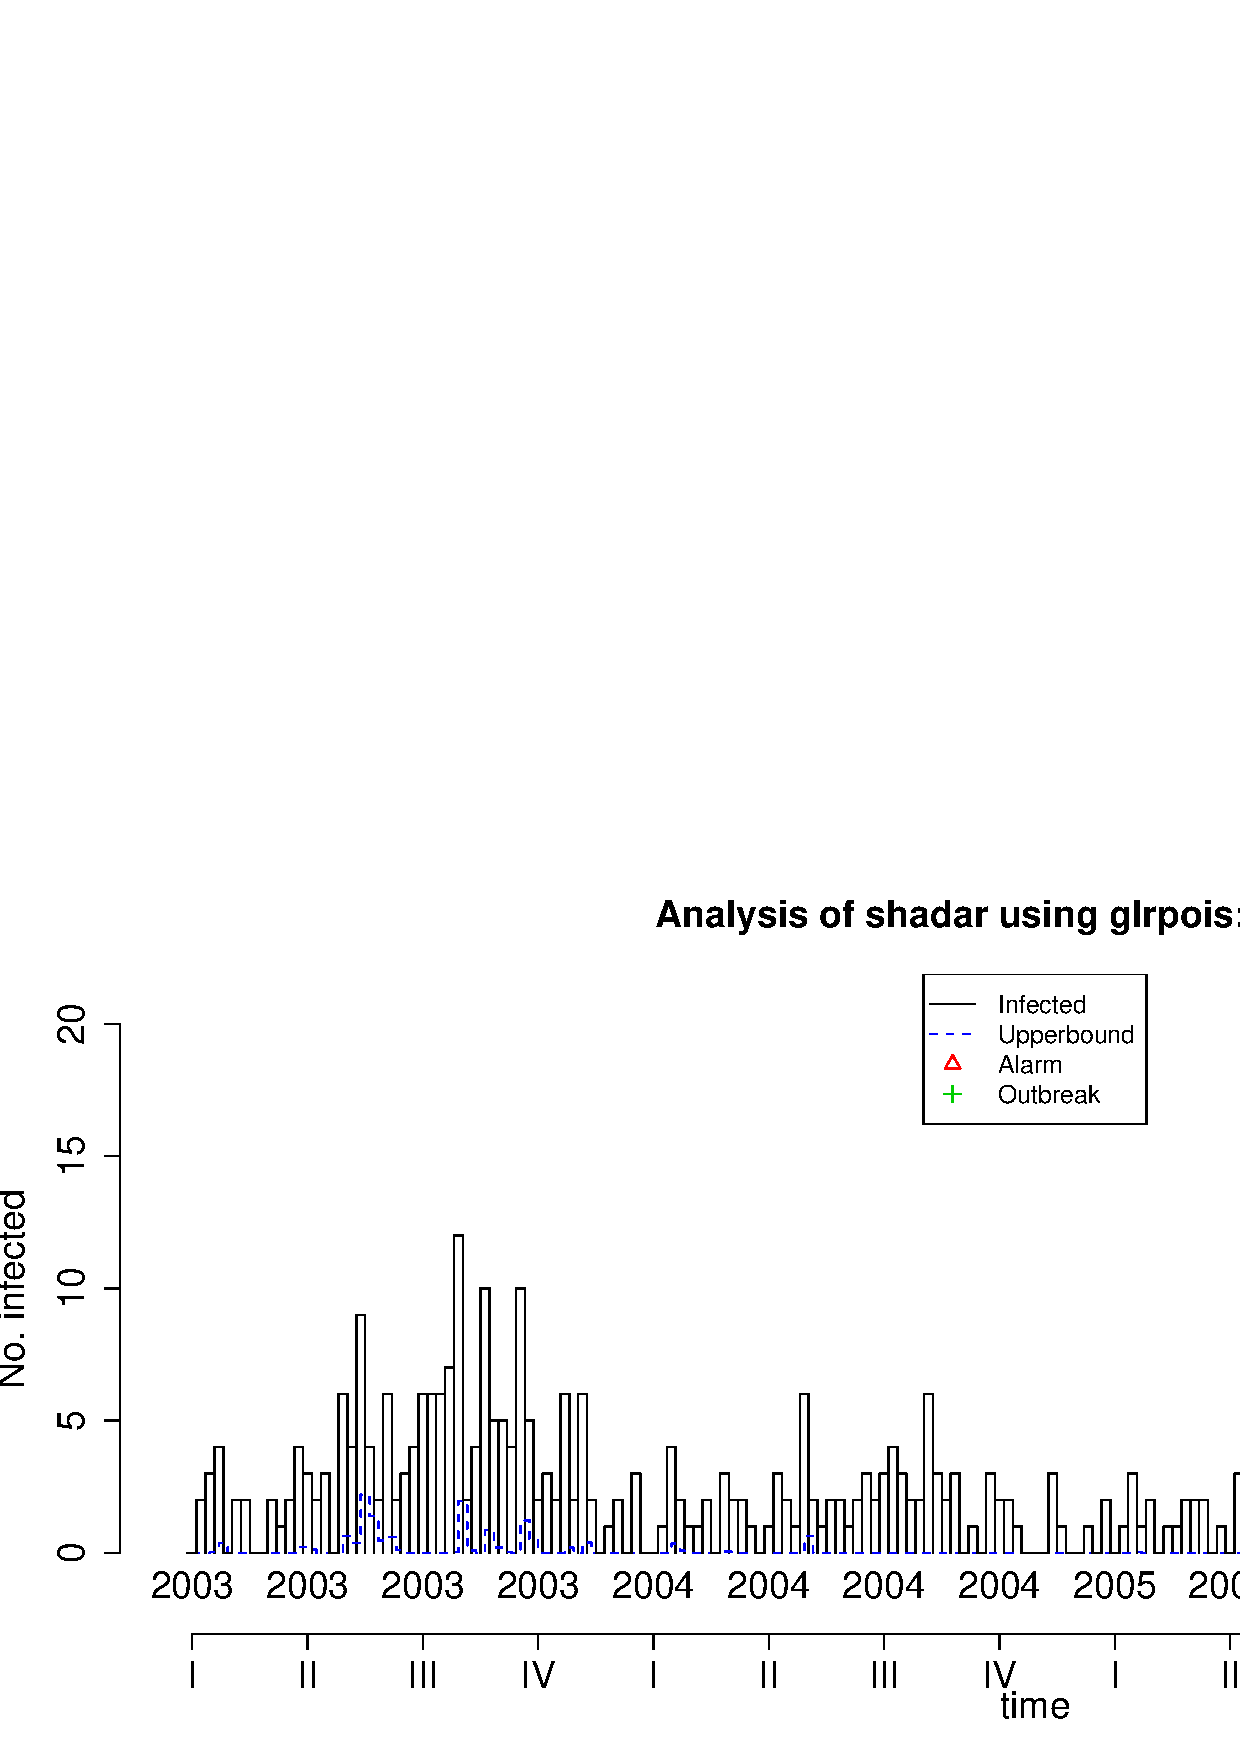
\includegraphics{figs/vignette_glrnb-005}

The default value for $c_{\gamma}$ is 5. The upperbound statistic is above this value several times in the third quarter of 2006 (time points marked by small triangles in the plot). 
In the next section follow a description of the control-setting for tuning the behavior of the algorithm, e.g.\ one can search not only for increases in mean as shown in the example but also for decreases.






   
\section{Control-settings}\label{sec:control}

In this section, the purpose and use of the control settings of the \verb+algo.glrnb+ function  are shown and illustrated by the examples from Section \ref{sec:prel}.


The control-setting is a list of the following arguments.

\begin{Schunk}
\begin{Sinput}
> control = list(range = range, c.ARL = 5, mu0 = NULL, 
+     alpha = 0, Mtilde = 1, M = -1, change = "intercept", 
+     theta = NULL, dir = c("inc", "dec"), ret = c("cases", 
+         "value"))
\end{Sinput}
\end{Schunk}


\begin{itemize}
\item \verb+range+ \\
The \verb+range+ is a vector of consecutive indices for the week numbers in the \verb+disProg+ object for which surveillance should be done. If a model for the in-control parameter $\mu_0$ is known (\verb+mu0+ is not \verb+NULL+), the surveillance can start at time point one. Otherwise it is necessary to estimate the values for \verb+mu0+ with a GLM. Thus, the range should not start at the first time point but instead use the first weeks/months as control-range. (Note: It is important to use enough data for estimating $\mu_0$, but one should be careful that these data are in control)

With the following call one uses the first 2 years (104 weeks) for estimating $\mu_0$ and the the years 2003 to 2006 will be on line monitored.
\begin{Schunk}
\begin{Sinput}
> control = list(range = 105:length(shadar$observed))
> algo.glrnb(disProgObj = shadar, control = control)
\end{Sinput}
\end{Schunk}

\item \verb+alpha+ \\
This is the (known) dispersion parameter $\alpha$ of the negative binomial distribution. If \verb+alpha+=0, modeling corresponds to the Poisson distribution. In this case, the call of \verb+algo.glrnb+ is similar to a call of \verb+algo.glrpois+. If $\alpha$ is known, the value can be specified in the \verb+control+-settings.

\begin{Schunk}
\begin{Sinput}
> control = list(range = 105:295, alpha = 3)
> algo.glrnb(disProgObj = shadar, control = control)
\end{Sinput}
\end{Schunk}

If overdispersion is present in the data, but the dispersion parameter $\alpha$ is unknown, an estimation $\hat{\alpha}$ is calculated as part of the in-control model estimation. Use \verb+alpha=NULL+ to get this estimation. 


The estimated value $\hat{\alpha}$ is saved in the \verb+survRes+-Object in the \verb+control+-list. Use

\begin{Schunk}
\begin{Sinput}
> control = list(range = 105:295, alpha = NULL)
> surv <- algo.glrnb(shadar, control = control)
> surv$control$alpha
\end{Sinput}
\begin{Soutput}
[1] 4.039254
\end{Soutput}
\end{Schunk}

to get the estimated dispersion parameter for the salmonella data.

\item \verb+mu0+ \\
This vector contains the values for $\mu_0$ for each time point in the \verb+range+. If it has the value \verb+NULL+  the observed values with indices 1 to \verb+range+-1 are used to fit a GLM. If there is no knowledge about the in-control parameter, one can use the values before the range to find an seasonal model as in equation \ref{mu0}. \verb+mu0+ is at the moment a list of three argument: \verb+S+ is the number of harmonics to include in the model, \verb+trend+ is Boolean whether a linear trend $\beta_1t$ should be considered. The default is to use the same model of $\mu_0$ for the whole surveillance. An alternative is, to fit a new model after every detected outbreak. If refitting should be done, choose \verb+refit=TRUE+ in the \verb+mu0+ list. In this case, the observed value from time point 1 to the time point of the last alarm are used for estimating a GLM. Then we get a new model after every alarm. 


In the following example a model with \verb+S+=2 harmonics and no linear trend is fitted for the Salmonella data. The observed cases from the first two years are used for fitting the GLM. 
   
\begin{Schunk}
\begin{Sinput}
> control = list(range = 105:295, mu0 = list(S = 2, trend = FALSE))
> algo.glrnb(disProgObj = shadar, control = control)
\end{Sinput}
\end{Schunk}


The predicted values for the in-control mean in the range are shown as a dashed line in the following plot.

\begin{Schunk}
\begin{Sinput}
> plot(shadar)
> with(surv$control, lines(mu0 ~ range, lty = 2, lwd = 4, 
+     col = 4))
\end{Sinput}
\end{Schunk}
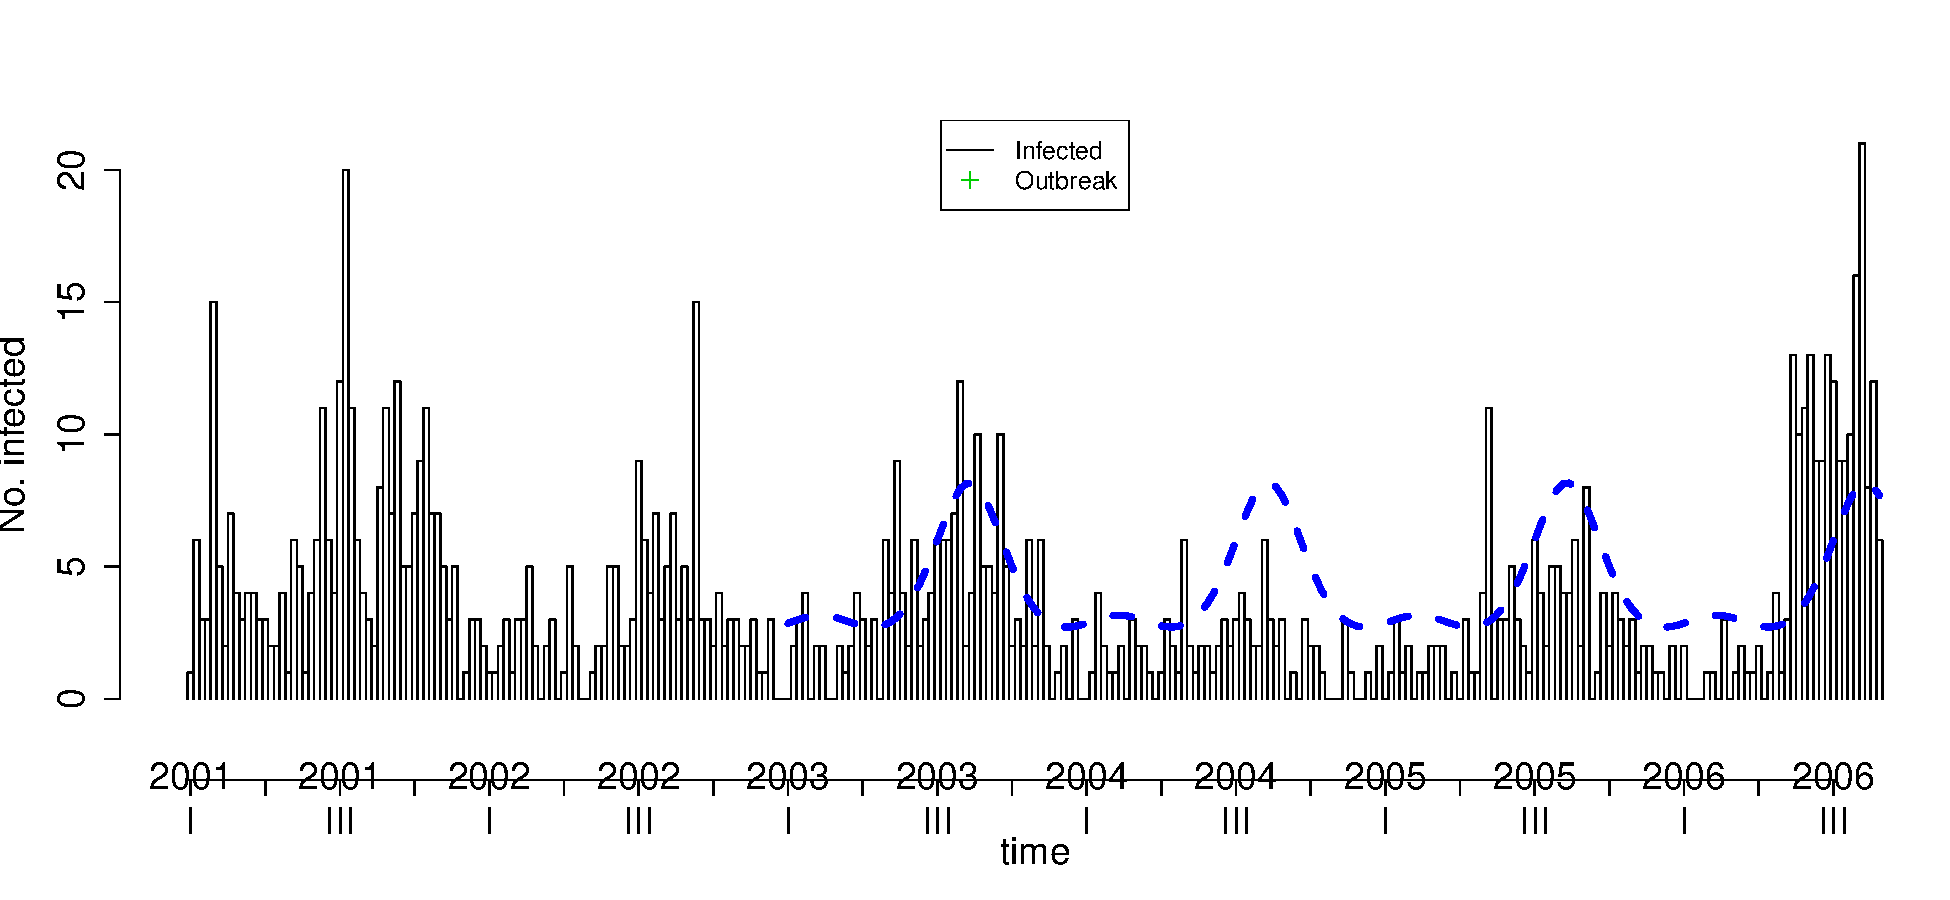
\includegraphics{figs/vignette_glrnb-012}


The information about the used model is saved in the \verb+survRes+-object, too. 

\begin{Schunk}
\begin{Sinput}
> surv$control$mu0Model
\end{Sinput}
\end{Schunk}

The $\mu_0$ model is fitted by a call of the function \verb+estimateGLRNbHook+. Instead of using the standard seasonal negative binomial model from equation \ref{mu0}, one can change the \texttt{R}-code of  the function \verb+estimateGLRNbHook+ to get any desired model. The standard code is the following

\begin{Schunk}
\begin{Sinput}
> estimateGLRNbHook
\end{Sinput}
\begin{Soutput}
function () 
{
    control <- parent.frame()$control
    p <- parent.frame()$disProgObj$freq
    range <- parent.frame()$range
    train <- 1:(range[1] - 1)
    test <- range
    data <- data.frame(y = parent.frame()$disProgObj$observed[train], 
        t = train)
    formula <- "y ~ 1 "
    if (control$mu0Model$trend) {
        formula <- paste(formula, " + t", sep = "")
    }
    for (s in 1:control$mu0Model$S) {
        formula <- paste(formula, "+cos(2*", s, "*pi/p*t)+ sin(2*", 
            s, "*pi/p*t)", sep = "")
    }
    m <- eval(substitute(glm.nb(form, data = data), list(form = as.formula(formula))))
    return(list(mod = m, pred = as.numeric(predict(m, newdata = data.frame(t = range), 
        type = "response"))))
}
\end{Soutput}
\end{Schunk}

To include own models in the \verb+estimateGLRNbHook+ function, the code of the function has to be changed. In the following code chunk \verb+estimateGLRNbHook+ is modified so that weights are included in the model.

\begin{small}
\begin{verbatim}
estimateGLRPoisHook <- function() {
  control <- parent.frame()$control
  p <- parent.frame()$disProgObj$freq
  range <- parent.frame()$range

  train <- 1:(range[1]-1)
  test <- range
  
  #Weights of training data - sliding window also possible
  weights <- exp(-0.3 * ((max(train)-train)) %/% 12)

  data <- data.frame(y=parent.frame()$disProgObj$observed[train],t=train)
  
  formula <- "y ~ 1 "
  if (control$mu0Model$trend) { formula <- paste(formula," + t",sep="") }
  for (s in 1:control$mu0Model$S) {
    formula <- paste(formula,"+cos(2*",s,"*pi/p*t)+ sin(2*",s,"*pi/p*t)",sep="")
  }
  

  m <- eval(substitute(glm(form,family=poisson(),data=data,weights=weights),
                       list(form=as.formula(formula))))
  return(list(mod=m,pred=as.numeric(predict(m,newdata=data.frame(t=test),   
  type="response"))))
}
\end{verbatim}
\end{small}



Additionally the fitted model from the call of \verb+estimateGLRNbHook+ is saved. The result of a call of \verb+glm.nb+ is in the standard setting an object of class \verb+negbin+  inheriting from class \verb+glm+. So methods as \verb+summary+, \verb+plot+ of \verb+predict+ can be used on this object. If refitting is done, the list of the used models is saved. Use 

\begin{Schunk}
\begin{Sinput}
> coef(surv$control$mu0Model$fitted[[1]])
\end{Sinput}
\begin{Soutput}
          (Intercept) cos(2 * 1 * pi/p * t) sin(2 * 1 * pi/p * t) 
          1.366509559          -0.330913468          -0.340248554 
cos(2 * 2 * pi/p * t) sin(2 * 2 * pi/p * t) 
         -0.008114547           0.259416100 
\end{Soutput}
\end{Schunk}

to get the estimated values of the first (and in case of \verb+refit=FALSE+ only) model for the parameter vector $\beta$ given in (\ref{mu0}).
 
\item \verb+c.ARL+ \\
This is just the threshold $c_{\gamma}$ for the GLR-test (see equation \ref{cusum}). The smaller the value is chosen, the more likely it is to detect an outbreak but on the other hand false alarms can be produced. 

\begin{Schunk}
\begin{Sinput}
> control = list(range = 105:295, alpha = 0)
> surv <- algo.glrnb(disProgObj = shadar, control = control)
> table(surv$alarm)
\end{Sinput}
\begin{Soutput}
  0   1 
185   6 
\end{Soutput}
\end{Schunk}

For a choice of $c_{\gamma}$ we get  6 alarms. In the following table the results for different choices of the threshold are shown.


\begin{table}[h]
\begin{center}
\caption{Number of alarms for salmonella hadar data in dependence of c.ARL}
\label{c.ARL}
\begin{tabular}{l|cccccc}
\verb+c.ARL+ & 1 & 2 & 3 & 4 & 5 & 6 \\
\hline
no. of alarms & 16 & 12 & 8 & 8 & 6 & 4
\end{tabular}
\end{center}
\end{table}





\item \verb+change+ \\
There are two possibilitys to define an outbreak. The intercept-change is described in Section \ref{sec:glr} and equation \ref{interceptchange}. Use \verb+change="intercept"+ to choose this possibility. The other alternative is the epidemic chart, where an auto-regressive model is used. See \citet{held2005} and \citet{hoehle2008} for more details. A call with \verb+change="epi"+ in the control-settings leads to this alternative. Note that in the epidemic chart not every feature of \verb+algo.glrnb+ is available. 

\item \verb+theta+ \\
If the change in intercept in the intercept-charts is known in advance, this value can be passed to the function (see Section \ref{sec:glr}). These LR-charts are faster but can lead to inferior results if a wrong value of \verb+theta+ is used compared to the actual out-of-control value (\citet{hoehle2008}). If  an increase of 50 percent in cases is common when there is an outbreak which corresponds to a $\kappa$ of $\log(1.5)=0.405$ in equation \ref{interceptchange} use

\begin{Schunk}
\begin{Sinput}
> control = list(range = 105:295, theta = 0.4)
> algo.glrnb(disProgObj = shadar, control = control)
\end{Sinput}
\end{Schunk}

If there is no knowledge about this value (which is the usual situation), it is not necessary to specify \verb+theta+. In the GLR-charts, the value for $\kappa$ is calculated by a maximation of the likelihood. Use the call   

\begin{Schunk}
\begin{Sinput}
> control = list(range = 105:295, theta = NULL)
> algo.glrnb(disProgObj = shadar, control = control)
\end{Sinput}
\end{Schunk}

in this situation.

\item \verb+ret+ \\
The \verb+upperbound+-statistic of a \verb+survRes+-object is usually filled with the LR- or GLR-statistic of equation \ref{cusum}. A small value means, that the in-control-situation is likely, a big value is a hint for an outbreak. If you choose \verb+ret="value"+, the upperbound slot is filled with the GLR-statistic. These values are plotted then, too. The alternative return value is \verb+"cases"+. In this case, the number of cases at time point $n$ that would have been necessary to produce an alarm are computed. The advantage of this option is the easy interpretation. If the actual number of cases is more extreme than the computed one, an alarm is given. With the following call, this is done for the salmonella data.

\begin{Schunk}
\begin{Sinput}
> control = list(range = 105:295, ret = "cases", alpha = 0)
> surv2 <- algo.glrnb(disProgObj = shadar, control = control)
\end{Sinput}
\end{Schunk}

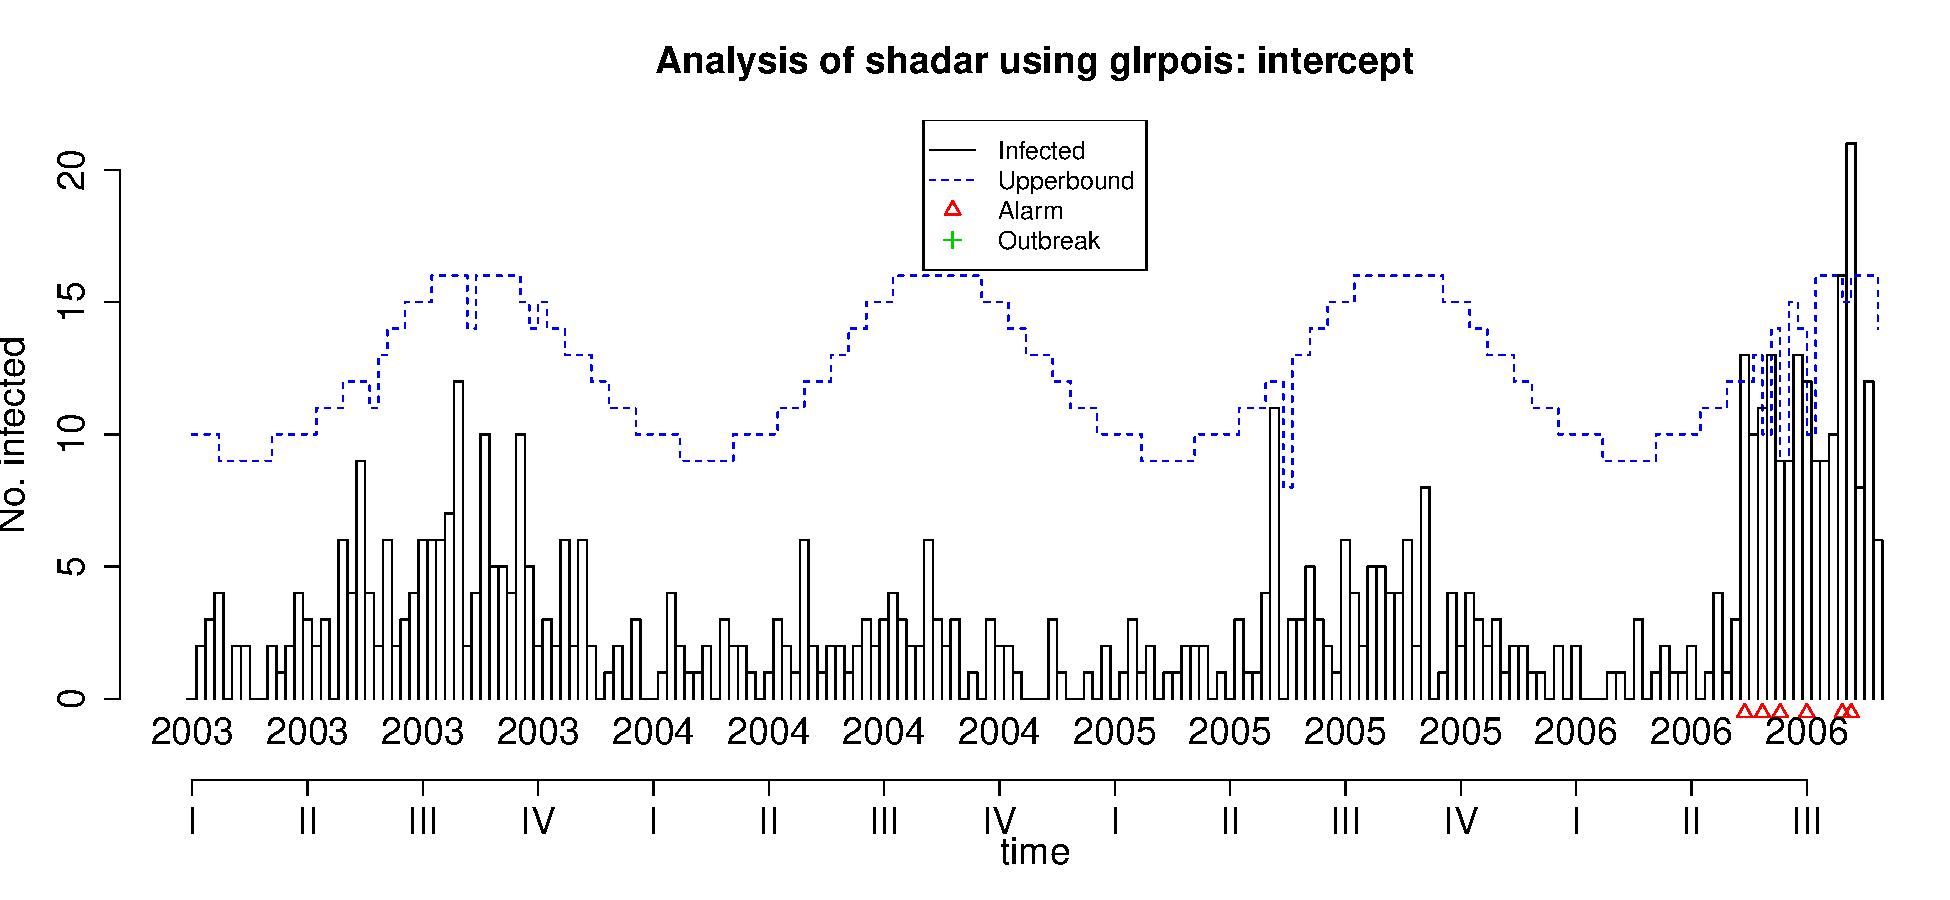
\includegraphics{figs/vignette_glrnb-021}

Of course, the alarm time points are the same as with \verb+ret="cases"+.

\item \verb+dir+ \\
In the surveillance of infectious diseases it is regular to detect an increase in the number of infected persons. This is also the standard setting for \verb+algo.glrnb+. But in other applications it could be of interest to detect a decrease of counts. For this purpose, the \verb+dir+-option is available. If \verb+dir+ is set to \verb+"inc"+, only increases in regard to the in-control mean are taken into account in the likelihood-ratio-statistic. With \verb+dir="dec"+, only decreases are considered.

As an example we take the salmonella data again, but know we look at the number of cases that would have been necessary if a decrease should be detected.

\begin{Schunk}
\begin{Sinput}
> control = list(range = 105:295, ret = "cases", dir = "dec", 
+     alpha = 0)
> surv3 <- algo.glrnb(disProgObj = shadar, control = control)
\end{Sinput}
\end{Schunk}

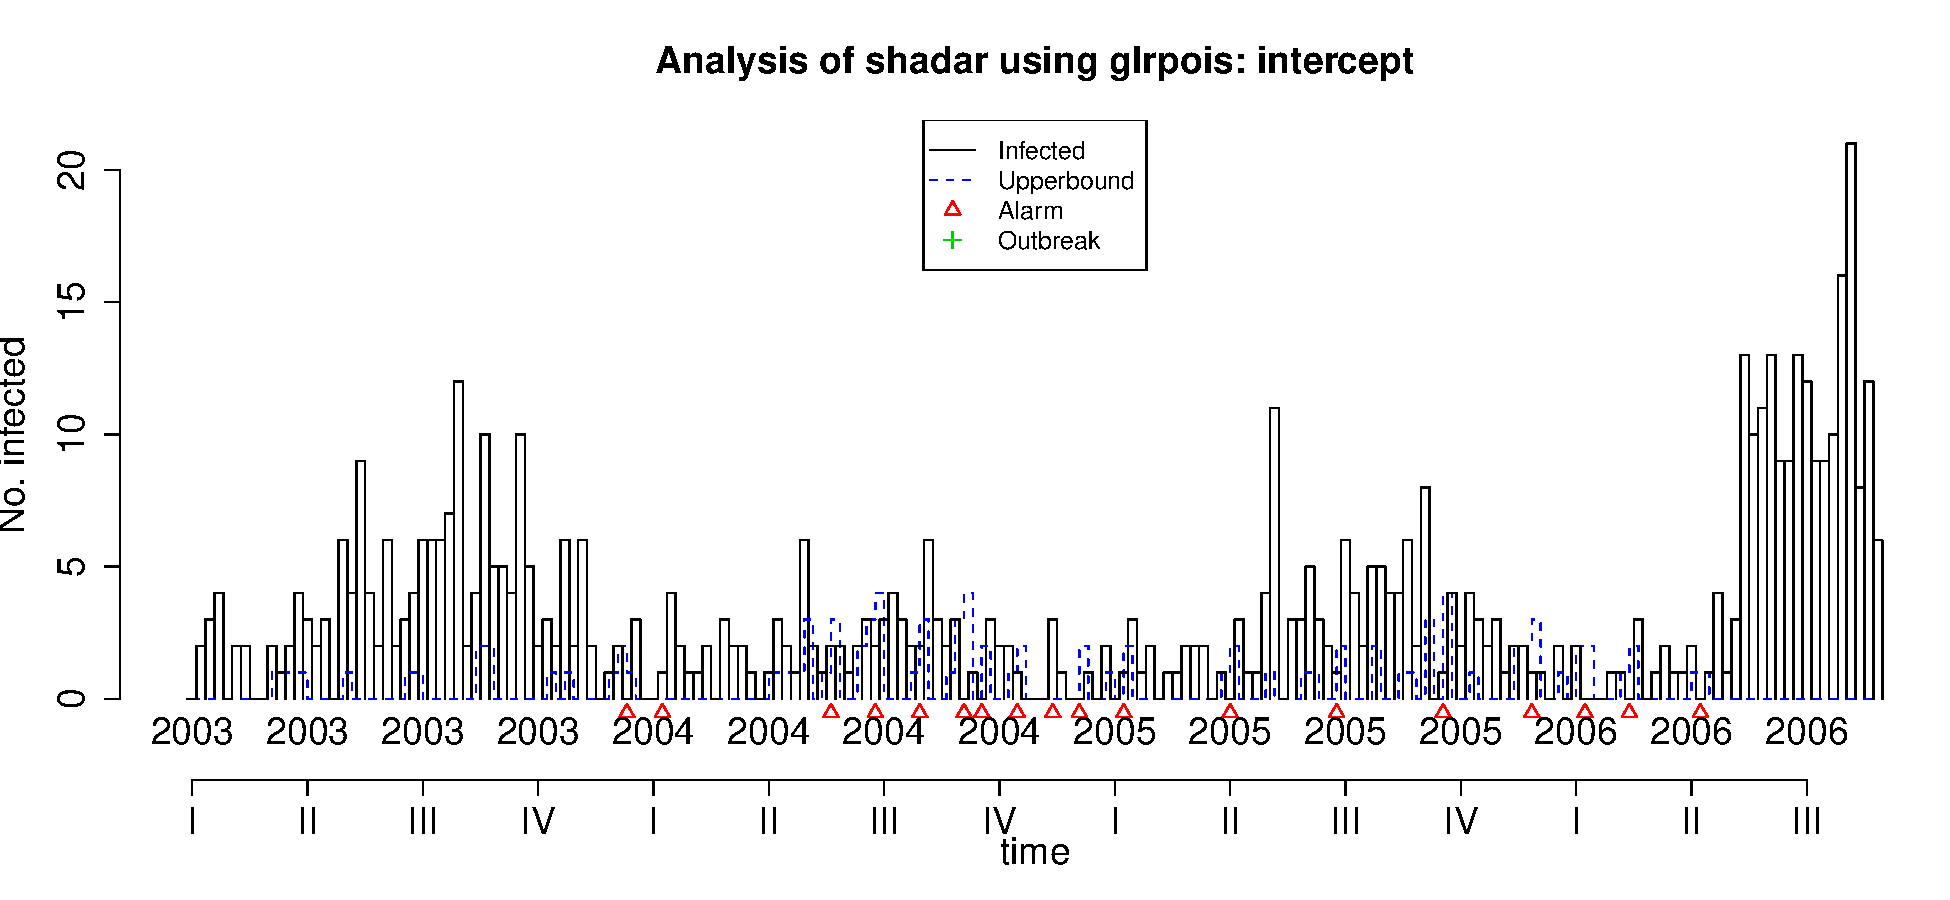
\includegraphics{figs/vignette_glrnb-023}

The observed number of cases is below the computed threshold several times in 2005 to 2006 and alarms are given.

\item \verb+Mtilde+ and \verb+M+ \\
These parameters are necessary for the so called ''window-limited'' GLR scheme. Here the maximation is not performed for all $1 \leq k \leq n$ but instead only for a window $k \in \{n-M,...,n-\tilde{M}+1 \}$ of values. Note that $1 \leq \tilde{M} \leq M$, where the minimum delay $\tilde{M}$ is the minimal required sample size to obtain a sufficient estimate of $\theta_1=(\mu_0,\kappa)$ ~\citep{hoehle2008}. The advantage of using a window of values instead of all values is the faster computation, but in the setup with intercept-charts and $\theta_1=\kappa$ this doesn't bother much and $\tilde{M}=1$ is sufficient.      
   

\end{itemize}

\section{Discussion}

As seen, the function \verb+algo.glrnb+ allows many possibilities for doing surveillance for a time series of counts. In order to achieve fast computations, the function is implemented in C. An important issue in surveillance is the quality of the used algorithms. This can be measured by the sensitivity and the specificity of the result. The aim of our future work is to provide the possibility for computing the quality and in the next step to include a ROC-approach in order to have a more formal framework for the choice of threshold $c_{\gamma}$. 



%\include{extensions}

%\renewcommand{\bibsection}{\section{REFERENCES}}
\bibliography{references}

\end{document}
